\documentclass[a4paper,10pt, twoside]{report}
\usepackage[utf8x]{inputenc}
\usepackage[T1]{fontenc}
\usepackage{titlesec, blindtext, color}
\usepackage{setspace}

\usepackage[hidelinks]{hyperref}

\usepackage[export]{adjustbox}
\usepackage{array}
\usepackage{color, colortbl}

\usepackage{float}
\usepackage{fancyhdr}
\usepackage{graphicx}
\usepackage[top=2cm, bottom=3cm, left=2.5cm, right=2.5cm]{geometry}

\usepackage[french]{babel}

\pagestyle{fancy}
\setlength{\headheight}{49pt}
\setlength{\footskip}{17pt}
% header
\fancyhead[R]{
\includegraphics[width=5cm]{logo_sciences.png}}
\fancyhead[L]{
\includegraphics[width=5cm]{logo_arksens.png}}

% footer
\fancyfoot[C]{Rapport de stage --- Master 2 FSIL\\Ludovic Lubeigt}
\fancyfoot[RO, LE] {\thepage}

% colors
\definecolor{gray73}{gray}{0.73}
\definecolor{arkred}{rgb}{0.592, 0.145, 0.168}

% commands
\newcommand{\hsp}{\hspace{20pt}}
\titleformat{\chapter}[hang]{\Huge\bfseries}
{\thechapter\hsp\textcolor{gray73}{|}\hsp}{0pt}{\Huge\bfseries}
\titleformat{\subsubsection}{}{}{}{\textbullet~}

\graphicspath{{images/}}

\begin{document}
\begin{spacing}{1.2}
 
% Page de garde
\begin{titlepage}
  \newgeometry{top=2cm, bottom=2cm, left=2cm, right=2cm}
  
  \begin{center}
    
\includegraphics[width=9cm]{logo_sciences.png}\\[2cm]
    
    \textsc{\bfseries\Large Rapport de stage\\[0.3cm]
    Master 2 -- Fiabilit\'e, S\'ecurit\'e et
    Int\'egration Logicielle\\[0.3cm]
        Parcours Fiabilit\'e et S\'ecurit\'e Informatique}\\[0.3cm]

    \rule{\linewidth}{1mm} \\[1cm]

    \textsc{\bfseries\huge Conception \&  d\'eveloppement syst\`eme de backup
    chiffr\'e et incr\'emental en C/C++}\\[1cm]

    \rule{\linewidth}{1mm}\\[1.5cm]

    \textsc{\huge Arksens Cyber Security}\\[2cm]
    
    \begin{figure}[H]
      \begin{minipage}[t]{8cm}
        \centering
        
\includegraphics[scale=0.50]{logo_adhara.png}
      \end{minipage}
      \begin{minipage}[t]{8cm}
        \centering
        
\includegraphics[width=7cm]{logo_arksens.png}
      \end{minipage}\\[1.3cm]
    \end{figure}
      
    \begin{minipage}{0.4\textwidth}
      \begin{flushleft} \large
        \emph{\bfseries Auteur :}\\
        Ludovic \textsc{Lubeigt}
      \end{flushleft}
    \end{minipage}
    \begin{minipage}{0.4\textwidth}
      \begin{flushright}
        \large \emph{\bfseries Tuteur Entreprise :}\\
        Ga\"etan \textsc{van Diemen}\\[0.2cm]
        \emph{\bfseries Enseignant :}\\
        Jean-Luc \textsc{Massat}
      \end{flushright}
    \end{minipage}\\[1.5cm]
      
    \large\emph{\bfseries Ann\'ee Universitaire :}\\
    2014 -- 2015

  \end{center}
\end{titlepage}

\begin{abstract}

Ce document pr\'esente le travail r\'ealis\'e lors du stage de fin d'\'etude
\`a Arksens Ltd. \`a l'\^ile Maurice entre le premier avril 2015 et le 25
septembre 2015 dans le cadre du Master 2 Fiabilit\'e et S\'ecurit\'e
Informatique \`a l'Universit\'e d'Aix-Marseille.

Le rapport est d\'ecoup\'e en deux parties. Une premi\`ere servant de rapport
de synth\`ese et pr\'esentant l'entreprise, le sujet de stage, le
travail effectu\'e de m\^eme que l'environnement de travail et les \'eventuelles
difficult\'es rencontr\'ees.
La seconde partie apporte un aspect technique au rapport et permet de 
pr\'esenter le travail r\'ealis\'e plus en d\'etail.
\end{abstract}

\newpage
\hfill
\section*{Remerciements}
Je tiens tout d'abord \`a remercier l'\'equipe p\'edagogique de la facult\'e des
sciences de l'universit\'e d'Aix-Marseille qui m'a permis d'avoir les
connaissances et les aptitudes n\'ecessaires au bon d\'eroulement de ce stage.

Je remercie \'egalement la soci\'et\'e Arksens pour m'avoir permis de faire mon
stage chez eux. Tout particuli\`erement, je remercie David Terranova et Ga\"etan
van Diemen qui m'ont accueilli \`a l'\^ile Maurice et suivi au jour le jour
durant ces six mois. Je n'oublie \'evidemment pas Micha\"el Colaone et le reste
de l'\'equipe pour l'accueil et la bonne ambiance au sein de l'entreprise.

Enfin je remercie toute les personnes que je peux oublier mais qui m'ont aid\'e,
dans l'\'ecriture de ce rapport, dans le cadre du stage ou qui m'ont tout
simplement fait d\'ecouvrir l'\^ile Maurice.

Je tiens tout particuli\`erement \`a remercier Sir Daniel Brands of House Brands,
the first of His Name, King of the Dutch, King of the flatlands and the first
Men, Breaker of Cars and Father of the Bikers.

\hfill
\tableofcontents
\thispagestyle{fancy}

\chapter*{Introduction}
\thispagestyle{fancy}
Dans le cadre du Master professionnel \textit{Fiabilit\'e, S\'ecurit\'e et
Int\'egration logicielle}, parcours \textit{Fiabilit\'e et S\'ecurit\'e
Informatique} \`a l'\textit{Universit\'e d'Aix-Marseille}, un stage de fin
d'\'etude doit \^etre effectu\'e en entreprise pour valider les acquis et
rentrer dans le monde professionnel.

J'ai r\'ealis\'e ce stage entre le 1\up{er} avril et le 25 septembre 2015, soit
une p\'eriode de six mois, \`a \textit{Adhara Cyber Security}, renomm\'ee 
\textit{Arksens} au 1\up{er} juillet.

Ce stage fut donc l'occasion pour moi de mettre en pratique mes connaissances,
acquises tout au long de mon parcours universitaire, dans un environnement
professionnel et de m'en servir pour mener au mieux la mission qui m'a
\'et\'e confi\'ee. En outre, j'ai d\^u cr\'eer \`a partir de rien un syst\`eme
de backup incr\'ementale et s\'ecuris\'e, offrant une encryption en local des
donn\'ees des utilisateurs. Ainsi m'a-t-il \'et\'e demand\'e de faire la
conception de ce projet dans un premier temps puis son d\'eveloppement dans un
second temps et ainsi voir le processus de cr\'eation, jusqu'\`a un stade
avanc\'e, de ce qui peut \^etre qualifi\'e de gros projet.

Ce rapport vient donc pr\'esenter le d\'eroulement du stage ainsi que le
travail accompli au sein de l'entreprise durant ces six mois.


\chapter{Rapport de synth\`ese}
\thispagestyle{fancy}
\section{Pr\'esentation de l'entreprise}
Cr\'e\'ee en 2013 et nomm\'ee alors \textit{Adhara Cyber Security} avant
d'\^etre renomm\'ee \textit{Arksens} au 1\up{er} juillet 2015, l'entreprise 
dans laquelle j'ai effectu\'e mon stage est sp\'ecialis\'ee en s\'ecurit\'e
informatique. se d\'eveloppe sur trois continents gr\^ace \`a une approche
novatrice et r\'epondant aux besoins des entreprises et administrations de
toutes tailles.

Le changement de nom a fait suite \`a une \'evolution des clients puisque
l'entreprise, bien que principalement prestataire de service pour des PME
s'est ouverte aux entreprises de taille plus importante. Revoyant leur
strat\'egie de commercialisation et de communication, l'entreprise se devait
donc de changer de nom.

\subsection{Pr\'esence dans le monde}
Aujourd'hui \textit{Arksens} est donc pr\'esent dans trois pays chacun sur
un continent diff\'erent (voir figure~\ref{mapArksens}) offrant ainsi aux
utilisateurs un service de proximit\'e :
\begin{itemize}
  \item Abu Dhabi aux \'Emirats Arabes Unis pour les activit\'es au Moyen
  Orient.
  \item Pamplemousses à l’\^ile Maurice pour les activit\'es africaines.
  \item Paris en France pour les activit\'es européennes.
\end{itemize}

\begin{figure}[h!]
  \centering
  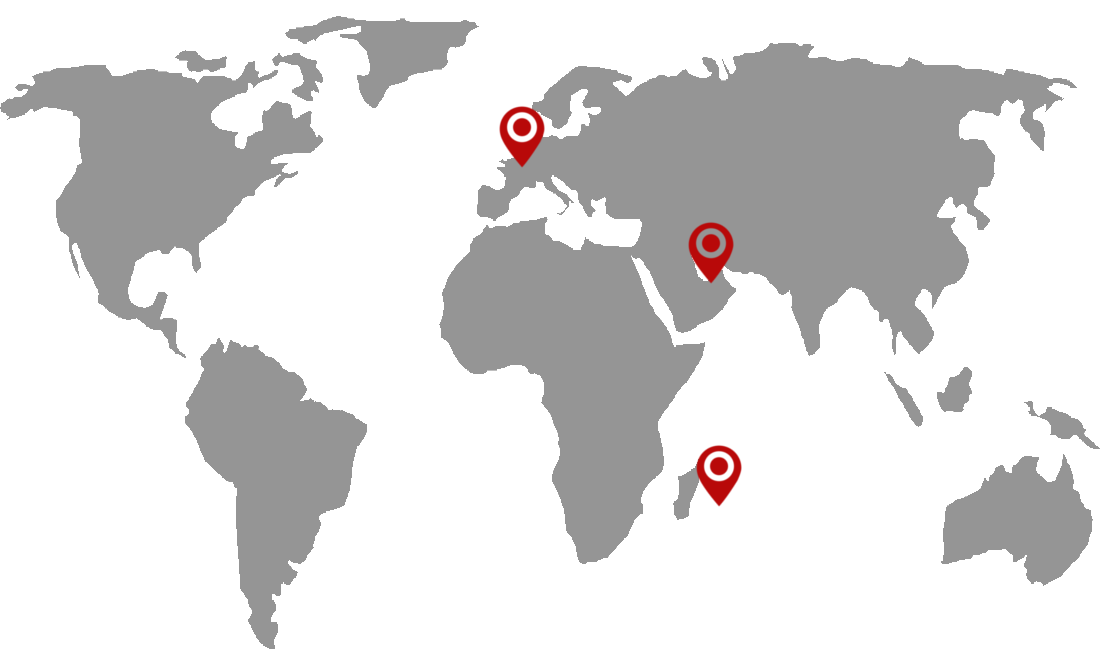
\includegraphics[scale=0.30]{map_arksens.png}
  \caption{\label{mapArksens} O\`u trouver Arksens}
\end{figure}
      
\subsection{Produits}
\textit{Arksens} propose aux entreprises 6 produits et solutions autour de la
s\'ecurit\'e informatique. Une rapide description de ces produits se trouve
table~\ref{tabProduits} :
\begin{table}[h!]
  \centering
  \def\arraystretch{1.5}
  \setlength{\fboxsep}{13pt} % padding
  \setlength{\fboxrule}{0pt} % frame
  \begin{tabular}{m{6cm}m{6cm}}
   \rowcolor{arkred} 
    \arrayrulecolor{gray73}\hline
    \color{white} \textbf{Produit} & \color{white} \textbf{Description} \\
    
\includegraphics[width=5cm, fbox]{produits/mail.png} & Prot\'eger l'information
    transitant par les mails. H\'ebergement de serveur email s\'ecuris\'e dans
    un cloud d\'edi\'e.\\
    \hline
    
\includegraphics[width=5cm, fbox]{produits/whisper.png} & Communications voix
    et images s\'ecuris\'es et anonymes.\\
    \hline
    
\includegraphics[width=5cm, fbox]{produits/backup.png} & Syst\`eme de
    chiffrement et de sauvegarde des donn\'ees dans un cloud d\'edi\'e.\\
    \hline
    
\includegraphics[width=5cm, fbox]{produits/gateway.png} & S\'ecuriser et
    rendre anonyme la navigation sur internet.\\
    \hline
    
\includegraphics[width=5cm, fbox]{produits/endpoint.png} & S\'ecuriser les
    postes utilisateurs en locales. C'est une ligne de d\'efense pour palier
    \`a la diffusion d'\'eventuels logiciels malveillants (virus, chevaux de
    Troie, vers, logiciels espions,\ldots{}) sur les ordinateurs et les
    serveurs.\\
    \hline
    
\includegraphics[width=5cm, fbox]{produits/nomad.png} & S\'ecuriser les
    donn\'ees personnelles sur appareils mobiles.\\
    \hline
  \end{tabular}
  \caption{\label{tabProduits} Produits et solutions par \textit{Arksens}}
\end{table}

L'ensemble des produits et solutions propos\'es par l'entreprise sont d\'ecrit
de mani\`ere plus compl\`ete sur leur site web~\cite{refArksens}.

\subsection{\^Ile Maurice}
Pour ma part, c'est l'\^ile Maurice qui m'int\'eresse puisque c'est l\`a o\`u
j'ai pass\'e ces six mois de stage. Les locaux, accueillant le centre de
recherche et d\'eveloppement de l'entreprise, se trouvent au Business Park de
Beau Plan (figure~\ref{beauPlan}) \`a Pamplemousses, ville situ\'ee au
nord-ouest de l'\^ile, \`a proximit\'e de Port Louis.

\begin{figure}[h!]
  \centering
  \includegraphics[width=15cm]{beau_plan_soir.jpg}
  \caption{\label{beauPlan} Beau Plan Business Park}
\end{figure}

L'\'equipe a beaucoup \'evolu\'ee entre mon arriv\'ee et mon d\'epart puisque
seulement trois personnes en plus du PDG, Micha\"el Colaone, \'etaient
pr\'esentent au 1\up{er} avril, date de d\'ebut du stage : David Terranova,
directeur des op\'erations, Ga\"etan van Diemen, chef de projet ainsi que
Daniel Brands, d\'eveloppeur web arriv\'e quelques jours auparavant.

L'\'equipe s'est agrandie par deux fois. D'abord \`a la mi-avril avec
l'arriv\'ee de deux autres stagiaire, Didier Mannone et
Yves Colin de Verdi\`ere, puis au 1\up{er} mai avec l'arriv\'ee d'Aymeric
Tabourin, ing\'enieur s\'ecurit\'e.

Bien que majoritairement francophone, la pr\'esence de personne d'origine
n\'eerlandaise a permis la cr\'eation d'un environnement international. Afin
de pouvoir communiquer avec l'ensemble des personnes de l'\'equipe,
l'utilisation de l'anglais au quotidien \'etait donc une n\'ecessit\'e.

L'int\'egration dans l'\'equipe fut donc facile et rapide et c'est donc dans
une bonne ambiance qu'\`a pu se d\'erouler ce stage de fin d'\'etude.

\section{Sujet de stage}
\subsection{Contexte}
L'entreprise \'etant encore jeune et de petite taille, plusieurs des services
existant \'etaient bas\'e sur des produits open source qui avaient \'et\'e
int\'egr\'e au \textit{manager}. Ce \textit{manager} est un environnement web
permettant aux utilisateurs de g\'erer les services auxquels ils ont souscrit
\`a partir d'un unique endroit et ainsi faciliter l'utilisation de ces derniers.

L'objectif de ce recrutement important \'etait pour l'entreprise de petit \`a
petit d\'evelopper ses propre logiciels et services afin de proposer aux
utilisateurs des produits adapt\'e et r\'epondant \`a leurs besoins sans passer
par des logiciels tiers.

C'est donc dans ce cadre que je suis arriv\'e et qu'il m'a \'et\'e demand\'e
de cr\'eer la prochaine g\'en\'eration de backup pour \textit{Arksens}.

\subsection{Le sujet}
Ma mission pour ce stage \'etait donc de faire la conception et le
d\'eveloppement d'un syst\`eme de backup incr\'emental et dont les donn\'ees
sauvegard\'ees sont chiffr\'ees en local, sur la machine client avant d'\^etre
envoy\'e sur des serveurs distant. Il me fallait donc d\'evelopper un
client/serveur multi plate-forme, robuste et s\'ecuris\'e r\'epondant \`a
la probl\'ematique suivante : combiner le chiffrement local avec la sauvegarde
incr\'ementale.

\`A mon arriv\'ee, David et Ga\"etan avait d\'ej\`a des id\'ees sur la
mani\`ere de r\'ealiser ce syst\`eme de sauvegarde, id\'ees que nous verrons
plus loin dans ce rapport. Et c'est \`a partir de celles-ci que j'ai pu
d\'emarrer mon travail, travail qui s'est divis\'e en trois grandes phases.

\begin{itemize}
 \item Phase de documentation et de r\'eflexion sur la probl\'ematique
 \item Conception logicielle
 \item D\'eveloppement
\end{itemize}

La premi\`ere phase, de documentation et de r\'eflexion, m'a permis de me
documenter dans un premier temps sur les diff\'erentes solution qui existe
d\'ej\`a puis de trouver un algorithme r\'epondant \`a la probl\'ematique.

La conception s'est faite en prenant en compte les contraintes existantes
et en se basant sur un travail de r\'eflexion d\'ej\`a effectu\'e par David et
Ga\"etan avant mon arriv\'ee.

Enfin, en ce qui concerne le d\'eveloppement, une des contraintes que j'avais
\'etait d'utiliser le C++ et de d\'evelopper de mani\`ere orient\'e objet tout
en faisant en sorte que le code puisse \^etre robuste, lisible, testable, et
donc facilement maintenable. De plus les librairies et framework utilis\'es
devaient \^etre sous licence libre.

Pour mener cette mission \`a bien, il avait \'et\'e d\'ecid\'e qu'une r\'eunion
hebdomadaire devait \^etre r\'ealis\'ee afin que David et Ga\"etan puissent
suivre l'avancement du projet mais aussi pour voir le travail effectu\'e la
semaine pr\'ec\'edente, essayer de r\'esoudre tout probl\`eme qui aurait pu
survenir et planifier la semaine suivante.
C'est en tout cas dans cette optique l\`a que nous avions commenc\'e. Dans les
fait, le retour des clients lors de mises \`a jour d'un produit ou des
r\'eunions avec les potentiels futur clients pouvait prendre la priorit\'e et
ainsi retarder ou annuler les r\'eunions hebdomadaire.

\section{D\'eroulement du stage}
\subsection{Travail de recherche}
\subsubsection{Documentation}
Mon travail de recherche s'est fait \`a partir d'une liste de mot cl\'e que
l'on m'a donn\'e afin quoi l'on parle tous le m\^eme langage. Entre autre,
certaines d\'efinitions li\'ees au backup et au chiffrement :
\begin{itemize}
 \item Backup incr\'emental
 \item Backup diff\'erentiel
 \item Transchiffrement
\end{itemize}

Mais aussi des logiciels d\'ej\`a existant, de backup ou de synchronisation de
fichiers et \`a partir desquels il peut \^etre int\'eressant de s'inspirer :
\begin{itemize}
 \item Syncthing~\cite{refSyncthing}
 \item rsync~\cite{refRsync}
\end{itemize}

\paragraph{Syncthing\\}
\textit{Syncthing} est un logiciel permettant la synchronisation des donn\'ees
entre plusieurs appareils de mani\`ere s\'ecuris\'ee gr\^ace \`a une
communication s\'ecuris\'ee via TLS. Les donn\'ees ne sont jamais stock\'ee
sur un serveur tiers, uniquement sur les diff\'erents ordinateurs utilis\'es.

Ce qui est int\'eressant dans \textit{Syncthing} est donc le protocole de
communication, qui a \'et\'e cr\'ee pour cela : Block Exchange Protocol (BEP)
~\cite{refBEP}. Ce protocole sous Creative Commons~\cite{refCC4.0}, est donc
une bonne source d'inspiration afin de faire la liaison entre notre client et
notre serveur.

\paragraph{rsync\\}
\textit{rsync} est un programme de transfert de fichiers pour les syst\`emes
Unix. Le c\oe ur du programme est son algorithme :
\textit{\flqq rsync algorithm \frqq}~\cite{refRsyncAlgo}.

Celui-ci va d\'ecouper un fichier en plusieurs blocs de taille identique et
calculer, pour chacun, un \texttt{checksum} ainsi qu'un \texttt{hash}. Ainsi,
pour n'envoyer que les parties modifi\'ees d'un ficher, l'algorithme va cr\'eer
une fen\^etre de la taille des blocs et la faire parcourir l'int\'egralit\'e du
fichier. Pour chaque position de la fen\^etre, si le \texttt{checksum} --- est
rapide \`a calculer mais dont le risque de collision est \'elev\'e ---
correspond au \texttt{checksum} d\'ej\`a calcul\'e d'un bloc, les \texttt{hash}
--- plus lent \`a calculer mais un risque de collision beaucoup plus faible, 
selon l'algorithme utilis\'e --- sont alors comparer. Si ceux-ci sont
identiques, la fen\^etre correspond \`a un bloc et tout ce qui pr\'ec\`ede ce
dernier, et jusqu'au pr\'ec\'edent bloc trouv\'e est une partie du fichier qui
a \'et\'e modifi\'e (ajout/modification/suppression) et est donc \`a
synchroniser.

C'est en grande partie cet algorithme qui m'a permis d'en trouver un qui me
permet de r\'epondre \`a ma probl\'ematique. Probl\'ematique \`a la fois
similaire puisqu'il fallait comparer deux fichiers distant pour ne trouver que
les diff\'erences mais diff\'erent dans la mesure o\`u il n'est pas possible
de maintenir dans mon cas une liste de bloc de m\^eme taille.

\subsubsection{R\'eflexion}
Une fois cette phase de documentation r\'ealis\'ee, il \'etait temps de trouver
un algorithme permettant d'identifier les parties d'un fichier ayant \'et\'e
modifi\'ee depuis le pr\'ec\'edent backup. Pour ce faire, et comme indiqu\'e
dans la partie documentation, je me suis bas\'e sur l'algorithme \textit{rsync}
pour, petit \`a petit, cr\'eer un algorithme qui permettait de r\'epondre \`a ma
probl\'ematique.

\paragraph{Chiffrement homomorphe\\}
Dans un premier temps, j'ai \'etudi\'e la question de l'homomorphisme. Ce type
de chiffrement permet de r\'ealiser des op\'erations sur des fichiers chiffr\'es
et de retourner le r\'esultat chiffr\'e. Ceci permet de faire des op\'erations
sans avoir \`a conna\^itre le contenu d'un fichier.

\begin{description}
 \item [Fonctionnement :] Dans notre cas, il nous aurait permis de concatener
 sur le serveur l'ensemble des morceaux d'un fichier avant de le re-d\'ecouper
 en bloc de taille \'egale puis de calculer pour chacun le \texttt{checksum}
 ainsi que le \texttt{hash}. Ceci aurait permis d'utiliser directement
 l'algorithme \textit{rsync} pour identifier les modifications faites sur un
 fichier.

 \item [Avantage :] Consommation de ressource et temps de calcul r\'eduit sur
 la machine client.
 
 \item [Inconv\'enient :] En utilisant le chiffrement homomorphe, le plus gros
 du calcul se fait sur le serveur entre deux backup, et ceux pour chaque
 fichier de chaque utilisateur. Ce type de chiffrement est donc tr\`es
 demandeur de ressource du c\^ot\'e du serveur pour que le programme fonctionne
 correctement.

 \item [Probl\`eme :] Le chiffrement homomorphe est un domaine de recherche
 tr\`es prometteur mais pas encore assez avanc\'e pour pouvoir \^etre utilis\'e
 en production. De plus le temps de calcul est extr\^emement \'elev\'e. Cette
 solution ne peut donc pas \^etre utilis\'ee aujourd'hui mais pourra peut-\^etre
 un jour \^etre envisag\'ee dans une prochaine version du backup.
\end{description}



\subsection{Conception}
\subsection{D\'eveloppement}

\newpage
\listoffigures
\listoftables
\bibliographystyle{abbrv-fr}
\bibliography{rapport_stage_arksens_2015}

\end{spacing}
\end{document}          